\documentclass[twoside]{article}
\setlength{\oddsidemargin}{0.25 in}
\setlength{\evensidemargin}{-0.25 in}
\setlength{\topmargin}{-0.6 in}
\setlength{\textwidth}{6.5 in}
\setlength{\textheight}{8.5 in}
\setlength{\headsep}{0.75 in}
\setlength{\parindent}{0 in}
\setlength{\parskip}{0.1 in}

%
% ADD PACKAGES here:
%

\usepackage{amsmath,amsfonts,amssymb,graphicx,mathtools,flexisym, hyperref,enumerate}
\usepackage[ruled,vlined]{algorithm2e}
\DontPrintSemicolon
\newcommand{\To}{\mbox{\upshape\bfseries to}}

% For images
\graphicspath{ {/assets/} }
%
% The following commands set up the lecnum (lecture number)
% counter and make various numbering schemes work relative
% to the lecture number.
%
\newcounter{lecnum}
\renewcommand{\thepage}{\thelecnum-\arabic{page}}
\renewcommand{\thesection}{\thelecnum.\arabic{section}}
\renewcommand{\theequation}{\thelecnum.\arabic{equation}}
\renewcommand{\thefigure}{\thelecnum.\arabic{figure}}
\renewcommand{\thetable}{\thelecnum.\arabic{table}}
\newcommand{\Lim}[1]{\raisebox{0.5ex}{\scalebox{0.8}{$\displaystyle \lim_{#1}\;$}}}
%
% The following macro is used to generate the header.
%
\newcommand{\lecture}[4]{
   \pagestyle{myheadings}
   \thispagestyle{plain}
   \newpage
   \setcounter{lecnum}{#1}
   \setcounter{page}{1}
   \noindent
   \begin{center}
   \framebox{
      \vbox{\vspace{2mm}
    \hbox to 6.28in { {\bf ECMT3170: Computational Econometrics
    \hfill } }
       \vspace{4mm}
       \hbox to 6.28in { {\Large \hfill #1. #2 \hfill} }
       \vspace{4mm}
       }
   }
   \end{center}


}
%
% Convention for citations is authors' initials followed by the year.
% For example, to cite a paper by Leighton and Maggs you would type
% \cite{LM89}, and to cite a paper by Strassen you would type \cite{S69}.
% (To avoid bibliography problems, for now we redefine the \cite command.)
% Also commands that create a suitable format for the reference list.
\renewcommand{\cite}[1]{[#1]}
\def\beginrefs{\begin{list}%
        {[\arabic{equation}]}{\usecounter{equation}
         \setlength{\leftmargin}{2.0truecm}\setlength{\labelsep}{0.4truecm}%
         \setlength{\labelwidth}{1.6truecm}}}
\def\endrefs{\end{list}}
\def\bibentry#1{\item[\hbox{[#1]}]}

%Use this command for a figure; it puts a figure in wherever you want it.
%usage: \fig{NUMBER}{SPACE-IN-INCHES}{CAPTION}
\newcommand{\fig}[3]{
            \vspace{#2}
            \begin{center}
            Figure \thelecnum.#1:~#3
            \end{center}
    }
% Use these for theorems, lemmas, proofs, etc.
\newtheorem{theorem}{Theorem}[lecnum]
\newtheorem{lemma}[theorem]{Lemma}
\newtheorem{proposition}[theorem]{Proposition}
\newtheorem{claim}[theorem]{Claim}
\newtheorem{corollary}[theorem]{Corollary}
\newtheorem{definition}[theorem]{Definition}
\newenvironment{proof}{{\bf Proof:}}{\hfill\rule{2mm}{2mm}}
\newtheorem{remark}[theorem]{Remark}


%
% To generate a clickable table of content.
%
\hypersetup{
    colorlinks,
    citecolor=black,
    filecolor=black,
    linkcolor=blue,
    urlcolor=black
}


\newcommand\E{\mathbb{E}}
\DeclareMathOperator*{\argmax}{arg\,max}
\DeclareMathOperator*{\argmin}{arg\,min}

\usepackage{tocloft}

\addtolength{\cftsecnumwidth}{10pt}
\setlength{\cftsubsecnumwidth}{3.5em}

\title{ECMT3170: Computational Econometrics}
\author{Charles Christopher Hyland}
\date{Semester 2 2018}


\begin{document}

\pagenumbering{gobble}
\maketitle
\begin{abstract}
Thank you for stopping by to read this. These are notes collated from lectures and tutorials as I took this course.
\end{abstract}
\newpage
\tableofcontents
\newpage
\pagenumbering{arabic}

%\lecture{**CHAPTER-NUMBER**}{**TITLE**}
\lecture{1}{Simulation Methods}

\section{Introduction to Simulation Techniques}
\section{Introduction to Simulation Techniques}
\subsection{Why Simulations?}

Before we begin, we first ask why do we even need computational techniques. An answer to this is that there are many reasons why we need computational techniques, as they can help us in scenarios such as
\begin{enumerate}[(i)]
  \item When we can't always trust asymptotic results in finite samples;
  \item When we can't trust assumptions underlying our models;
  \item When we want to run methods that have not been coded up.
\end{enumerate}

Furthermore, on the topic of simulations, we need simulations when we need to be able to generate draws from distributions. There are many practical applications to this such as simulating random terms in time series $\epsilon_i$, constructing random samples, and more. However, sampling from distributions other than the uniform tend to be quite difficult, due to many reasons as we will soon discover. Furthermore, when you construct distributions yourself that are not currently written in Python or R, it is useful to write your own methods to sample from your own distributions. 


We look at some examples of computational techniques. Alot of times we require computational techniques for expressions that do not have analytical expressions. In particular, we focus on 2 techniques, simulation and numerical integration. 


\subsection{Numerical Integration}
We have a function h(x) which we seek to evaluate at a grid of points $x_i$. We then use those values to approximate h by a $\textbf{piecewise linear function}$, which we can integrate $\textit{exactly}$ in order to find an approximation to $\int_{x \in \mathbb{D}}h(x)dx$. Keep this integral in mind as we will spend the rest of this chapter on finding out how to evaluate this integral. Such examples of this include both midpoint and trapezoid rule. These algorithms converge quickly in low dimension with bounded domains.
\begin{center}
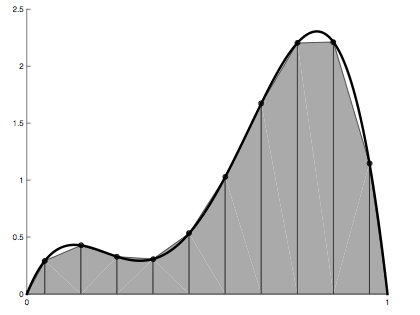
\includegraphics[width=3cm, height=4cm]{assets/trapezoid.png}

(Trapezoid Rule)
\end{center}
\begin{center}
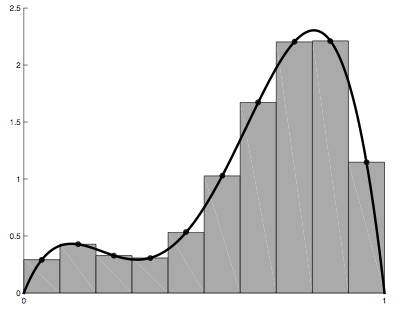
\includegraphics[width=3cm, height=4cm]{assets/midpoint.png}

(Midpoint Rule)
\end{center}

The issue is for high-dimensional problems, we suffer from the $\textbf{curse of dimensionality}$, as we try to cover too much of the space. Hence, such techniques do not scale well. For example, if we get 4 grid points for each dimension, so only 4 points along each axis, we would already have $4^{10}$ points to sample and that is already massive for such a poor performance. Instead, sampling random points is more efficient, that is, if the space was $\mathbb{R}^{10}$, we would sample vectors with 10 components and evaluate them accordingly. The issue is that this does not work really well. Hence, we turn to Monte Carlo integration instead.


\subsection{Monte Carlo Integration}
Recall that expectations for density functions of continuous random variables are just integrals, hence, we try to write our integrals as an expectation. Then finding the expectation is equivalent to evaluating the integral, except that computing expectations are much easier to do.

First we need to recall some properties of density functions f, on the domain $\mathbb{D}$.
\begin{enumerate}[(i)]
  \item f is never negative;
  \item $\int_{x \in \mathbb{D}}f(x)dx = 1$;
  \item Some properties of smoothness. 
\end{enumerate}

Then, we need to recall the $\textbf{Law of the Unconscious Statistician}$ that states that if we want to calculate the $\textbf{expected value}$ of a function g(X) for the random variable X, if we know the probability distribution of X but not g(X), we can simply compute 
$$
\mathbb{E}(g(X)) = \int_{\infty}^{\infty}g(x)f_X(x)dx
$$ 
and this still works in giving us the expectation of g(X).

So now, if we are interested in evaluating the integral
$$
\int_{x \in \mathbb{D}}h(x)dx
$$
we re-express h(x) as
$$
h(x) = v(x)f(x)
$$
where f(x) is a density function on the domain $\mathbb{D}$ and then we simply define v to be $\frac{h}{f}$.

Bringing it all together, we have that 
$$
\int_{x \in \mathbb{D}}h(x)dx = \int_{x \in \mathbb{D}}v(x)f(x)dv = \mathbb{E}[v(X)]
$$
where X is a random variable with density function f. Furthermore, the last equality is just the application of LOTUS. Hence, we have just written our integral of h(.) as an expectation of a random variable X, with a density function f(.), that relates to h(.). 

For a quick high level overview, since we need to find $\mathbb{E}[v(X)]$ in order to compute the integral of h(.), recall that expectations are simply averages, so all we need to do is sample multiple v(x) for $x \in \mathbb{D}$ (over the same domain as the integral of interest h), and simply take the average of these v(x) values. We have just computed $\mathbb{E}[v(X)]$ and therefore the integral of h(x)! In particular, what we do is that we take draws $x_1, x_2, ..., x_S$ from the distributioin with the density function $\mathbf{f}$ and then apply the function v(.) to each of those samples and then take the average so that we have
$$
\mathbb{E}[v(X)] = \frac{1}{S}\sum_{i=1}^Sv(x_i).
$$
So we take draws from the distribution with the density f and evaluate v(.) on it.

In particular, we hope that the distribution with the density f() that we have chosen is one that is very easy to sample from. From this, we can have multiple draws from that distribution and therefore the expectation of v(.). 

The pseudocode for this is

\begin{algorithm}
\DontPrintSemicolon
\KwIn{Draws of sampled $x_i$ from distribution with PDF f.}
\KwOut{Integral of function of interest h(.).}
$S \gets$ specified by user\;
$i \gets 0$\;
\While{$i < S$}{
  $x_i \gets $ draw from distribution with PDF f\;
  $v_i \gets v(x_i)$\;
  $i \gets i + 1$
}

$integral \gets Average(v_i)$

\Return{integral}\;
\caption{{\sc Monte Carlo Integration}}

\end{algorithm}

In terms of theoretical justifications for this, recall that the $\textbf{weak law of large numbers}$ (Khinchin's Law) states that the sample average $\textbf{converges in probability}$ towards the expected value for a sequence of random variables that are i.i.d and whose first moment exists. Convergence in probability is that the probability of an unusual outcome becomes smaller and smaller as the sequence progresses, or in other words
$$
\Lim{n \rightarrow \infty}Pr(|X_n - X| > \epsilon) = 0
$$

for a sequence of random variables $\{X_n\}$ and all $\epsilon > 0$. Therefore, the WLLN can then be expressed as
$$
\Lim{n \rightarrow \infty}Pr(|\bar{X}_n - \mu| > \epsilon) = 0,
$$

where $\mu$ is the expected value and $\bar{X} = \frac{1}{n}(X_1 + ... + X_n)$. Hence, going back to our scenario, as long as $v(x)$ is a sequence of Lebesgue integrable random variables (which means that their expected value exists and is finite), we have that
$$
\frac{1}{S}\sum_{k=1}^Sv(x^{(s)}) \rightarrow E[v(X)] = \int_{X \in \mathbb{D}}h(x)dx.
$$

Hence, we see that this converges to our integral of interest as number of draws from f increases or $S \rightarrow \infty$. An important thing to note is that unlike most cases of asymptotics, we actually have control over S and hence we can keep simulating to ensure we get the integral of interest! We have consistency here. 

Furthermore, invoking the Central Limit Theorem (the normalized sum of independent random variables tend towards a normal distribution), if the second moment is finite, Var[v(x)], then we have that
$$
\sqrt{S}\big(\frac{1}{S}\sum_{s=1}^Sv(x^{(s)})\big) - \int v(x)f(x)dx) \xrightarrow{d} \mathcal{N}(0, Var[v(x)])
$$
where we have convergence in distribution as $S \xrightarrow{d} \infty$. Here, note that we have the same convergence rate of $\sqrt{S}$ as in other cases, except that here we can actually control S! 

Additionally, we also now have a $\textbf{standard error}$ on our approximation, which is 
$$
SE = \sqrt{\frac{Var[v(x^{(s)})]}{S}}
$$
As S in the denominator, increasing the number of draws S actually decreases the standard error! The antithetic section will have more information on how to go about increasing draws efficiently. Hence, increasing S should decreases the standard error by $\sqrt{S}$. 


\subsection{Sampling from Distributions}
We see that we need the ability to sample from distributions in order for our Monte Carlo integration technique to work. 

First, we require an ability to sample from a uniform random variable $\mathbb{U}(0,1)$. To generate these uniform random variables, we use the deterministic recursive sequence of

$$
X_{i+1} = aX_i + c(\text{mod m}),
$$

where the initial value $X_0$ is the $\text{seed}$, a is the multiplier, c the increment, and m the modulus (and m is generally a large prime number). If we run this n times, we will have generated n random numbers. Then, we define $U_i = \frac{X_i}{m}$ for all i = 0,...,n and from this, we have generated n uniform random variables.

We now take it for granted that we can already sample from the standard uniform $\mathbb{U}(0,1)$ and Gaussian $\mathcal{N}(0,1)$ distributions. We can scale and shift these random variables in order to generate new ones. An example is that $\chi^2$ distribution is the sum of squared normals. Hence, to get $\chi^2$ with n degrees of freedom, generate n independent standard normal draws $z_i$ and compute $\sum_{i=1}^2z_i^2$. Additionally, the t distribution is defined to be $\frac{Z}{\frac{\sqrt{Y}}{n}}$ where Z is standard normal and Y is $\chi^2$ random variable.

In the cases of where we want to simulate from multivariate normal distribution of $X \sim \mathcal{N}(\mu, \Sigma)$, we can generate n $Z_i$ independent univariate standard normal random variables. Hence, to get a multivariate normal distribution $X \sim \mathcal{N}(\mu, \Sigma)$, we simply go 
$$
A + BZ \sim \mathcal{N}(A, BB^T),
$$
where $A = \mu$ and B is a matrix such that $BB^T = \Sigma$, where the Cholesky factor helps to find this. 

\subsection{Inverse CDF Method}
A general technique for transforming from standard uniform to distribution with CDF F is to compute $F^{-1}(u)$ and then apply it to a uniform random variable.

\begin{definition}
(Inverse CDF). 

$$
F^{-1}(u) = inf\{x|F(x) \geq u\}.
$$
\end{definition}

\begin{theorem}(Inverse CDF Method). 

Let $U \sim \mathbb{U}(0,1)$ and $X = F^{-1}(U)$, then $X \sim F$.
\end{theorem}

\begin{proof}
$$
P(X \leq x) = P(F(X) \leq F(x))
$$
$$
= P(F(F^{-1}U)\leq F(x))
$$
$$
= P(U \leq F(x))
$$
$$
= F(x).
$$
As F() is strictly increasing, $X \leq x$ is equivalent to $F(X) \leq F(x)$. The last equality follows from that the standard uniform distribution has a CDF is equal to $P(U \leq u) = u$ for $0 < u < 1$.
\end{proof}

This technique fails when it is hard to compute the inverse CDF, as it requires alot of work at times to compute.

\subsection{Acceptance/Rejection Method}

%http://www.columbia.edu/~ks20/4703-Sigman/4703-07-Notes-ARM.pdf

We have a distribution F in which we want to sample from but previous techniques we mentioned does not work. An example would be that we are unable to find an explicit formula for $F^{-1}()$. 

The intuition for the acceptance/rejection method is to sample from a different distribution G which we can sample from. We then reject draws from this that are more likely to be from G. The remaining draws we have are most likely to be from F. Hence, we accept some draws and reject others. Intuitively, we want G to be similar to F or else we end up rejecting alot of draws and waste time.

Hence, from distribution G with density g, we seek to approximate our distribution of interest F, with density f. We require that there exists a known and finite number $c>0$ such that
$$
sup\{\frac{f(x)}{g(x)}\} \leq c
$$
for all x in the support of F, $\mathbb{D}$. In particular, we seek this constant c to be as close to 1 as possible, as this means the density functions f and g are very similar.

The number of iterations N required for the algorithm is itself a random variable and has a geometric distribution as we wait until we have a successful draw. This geometric distribution has a success probability $p = P(U \leq \frac{f(Y)}{c.g(Y)})$. Therefore, we have that $P(N=n) = (1-p)^{n-1}p$, for $n \geq 1$. Hence, the expected number of iterations expected is
$$
E(N) = \frac{1}{p}.
$$
From this, we can compute what the parameter p is by conditioning on Y. Recall that for the CDF of a uniform random variable
$$
P(U \leq \frac{F(Y)}{c.g(Y)}|Y=y) = \frac{f(y)}{c.g(y)}
$$
where note that we have y instead of Y as we conditioned on Y=y.  Hence, we have that
$$
p = P(U \leq \frac{f(Y)}{c.g(Y)}) = \int_{- \infty}^{\infty}\frac{f(y)}{c.g(y)}\;g(y)\;dy
$$
$$
= \frac{1}{c}\int_{\infty}^{\infty}f(y)\;dy
$$
$$
= \frac{1}{c}.
$$
Hence, we have that $p = \frac{1}{c}$, which then imples that $E(N) = \frac{1}{p} = \frac{1}{1/c} = c$. This means that it takes on average c draws to accept one draw of x. Hence, we want the smallest c possible to minimise the number of draws and this only occurs if $\textbf{f and g are similar}$.

Hence, the algorithm for drawing just $\textbf{one}$ sample from distribution F is stated below.

\begin{algorithm}
\DontPrintSemicolon
\KwIn{Draws of sampled y from distribution G.}
\KwOut{Approximate a draw from distribution F.}
$y \gets $ draw from distribution G\;
$u \gets $ draw from uniform distribution U\;

\While{True}{

  \uIf{$u \leq \frac{f(y)}{c.g(y)}$}{
    $x \gets y$\;
    break\;
  }
  \Else{
    Continue
  }
}
\Return{x}\;
\caption{{\sc Acceptance/Rejection Method}}
\label{algo:duplicate}
\end{algorithm}

We can simply set a while loop counter if we wanted to certain a sample of size N from F. 

\subsection{Applications of acceptance/rejection methods}

\textbf{Truncated Distribution}


\begin{definition}(Truncated Distribution). 

Let X be a random variable distributed according to a PDF f, alongside a CDF F with infinite support. The probability density of the random variable after restricting the support such that $a < X \leq b$, has a conditional PDF of
$$
f(x|a<X \leq b) = \frac{g(x)}{F(b) - F(a)}
$$
where g(x) = f(x) for all $a < x \leq b$ and g(x) = 0 everywhere else. This is known as the truncated distribution of X on the support y=(a,b].
\end{definition}

\bigskip

\textbf{Discrete Distribution}
Suppose we want to draw an x such that
\[x = \begin{cases}
    
    0 \;\; prob=\frac{1}{3}\\
    1 \;\; prob=\frac{2}{3}\\
    \end{cases}
\]
but we only have a fair coin, which we draw y with 0.5 probability for 1 or 0 respectively. 

We need to find a c such that $f \leq c.g$. Hence, we solve for $\frac{f}{g} \leq c$. 

\[c = \begin{cases}
    
    \frac{1/3}{1/2} = \frac{2}{3} \;\;\; x=y=0\\
    \frac{2/3}{1/2} = \frac{4}{3} \;\;\; x=y=1\\
    \end{cases}
\]
Taking the maximum, the minimum that c has to be is $\frac{4}{3}$. Any c larger than this slows the algorithm down. 

Now, if y=0 is drawn (where probability = 0.5) and we sample a draw from the (0,1) uniform, the probability of acceptance is
$$
P(u \leq \frac{1/3}{4/3 . 1/2}) = \frac{1}{2}.
$$
Hence, the overall probability that we get a draw of x = 0 is the probability of a draw of y=0 multiplied by we accept it, hence 0.5*0.5 = 0.25. 

For y=1 with probability 0.5, we have that 
$$
P(u \leq \frac{2/3}{4/3 . 1/2}) = 1.
$$
Hence, the overall probability that we get a draw of x = 1 is the probability of a draw of y=1 multiplied by we accept it, hence 0.5*1 = 0.5. 

Therefore, the probability of rejecting a draw is (1-0.5-0.25) = 0.25. Hence, the conditional distribution of sampling an x with the probabilities that we specified is satisfied as

\[x = \; \begin{cases}
    
    0\;\;\; \text{with prob} = \frac{1/4}{1/4 + 1/2} = \frac{1}{3}\\
    1\;\;\; \text{with prob} = \frac{2/4}{1/4 + 1/2} = \frac{2}{3}\\
    \end{cases}
\]


Note that if the densities of g and f are different, then this technique won't work well as the standard errors will be large due to $\frac{h}{f}$ acting up and hence inflating our variance.


\section{Reducing noise in our draws}
\subsection{Antithetic Acceleration}

An issue is that when we simulate lots of draws, introduces noise into our model. We find ways to reduce the number of draws needed.

Recalling the section on Monte Carlo integration, to decrease the standard error, we can simply take more draws! In particular, if we have 2 unbiased estimators, the average of them is also an unbiased estimators. If they have the same variance with a correlation of $\rho$, you can see that
$$
Var(\frac{1}{2}(\hat{\theta}_1 + \hat{\theta}_2)) = \frac{\sigma^2}{2}(1 + \rho).
$$
Hence, if we find unbiased estimators that are negatively correlated, this can actually reduce the variance without needing to increase the number of draws S. 


From this, we can use antithetic acceleration to help us. In this case, an estimator with the same mean and variance as the sample average of $v(x^{(s)})$, is the sample average of the symmetric draws of $x^{(s)}$. In particular, if U is drawn from a uniform, taking 1-U also has the same distribution. If Z is drawn from normal, then -Z has the same distribution. Hence, we can have 2 sets of draws of x where the other set is a transformation applied such that we get the same distribution. Therefore, antithetic acceleration for our Monte Carlo integration is
$$
\frac{1}{2}\left(\frac{1}{S}\sum_{s=1}^Sv(x^{(s)}) + \frac{1}{S}\sum_{s=1}^Sv(x^{*(s)})\right)
$$

This especially powerful for the inverse CDF method, as recall that we are simply sampling from the uniform distribution, and hence 1-u is also a legitimate draw as well.

\subsection{Importance Sampling}
Importance sampling builds upon the acceptance/rejection method, where we want to sample from the distribution F but we can only sample from the distribution G. Now instead of rejecting bad draws, we can simply give them a lower weight when defining our estimator, which is reasonable if the density f has a distribution that is difficult to sample from. Hence, if a draw from a region that is more likely to be from G than F, we give it a smaller weight, which we define the weight to be $\frac{f(x^{(s)})}{g(x^{(s)})}$. In particular, we specify another PDF that is easier to sample from.

We want to have a function g that is $g \approx f$ just like in the acceptance/rejection method. However, we now no longer require that $f \leq c.g$, the only thing we require is that g is positive where f is. In other words, they have the same support. PDFs are never negative and hence we do not need to concern ourselves with that case. 

We want to estimate 
$$
\int v(x)f(x)dx
$$
which is the distribution F. Recall that since f is a density, $\int f(x)dx = 1$. Therefore, through manipulation, we have that

$$
\int v(x)f(x)dx = \frac{\int v(x)f(x)dx}{\int f(x)dx}
$$

then for a g that is positive for wherever f is positive, we have that 

$$
= \frac{\int v(x)\frac{f(x)}{g(x)}g(x)dx}{\int \frac{f(x)}{g(x)}g(x)dx}.
$$

Looking at only the numerator as the denominator is just equal to 1, we then define $w = \frac{f}{g}$. If $X \sim G$, then we have

$$
\int \frac{f(x)}{g(x)}g(x)dx = E[w(X)],
$$
as a result of the Law of the unconcious statistician. From this, we have that 

$$
\int v(x)\frac{f(x)}{g(x)}g(x)dx \; = \; \mathbb{E}[\frac{v(X)f(X)}{g(X)}] \; = \; \mathbb{E}[v(X)w(X)].
$$
Through the Law of Large numbers, we have that
$$
\hat{\theta} = \frac{1}{S}\sum_{s=1}^{S}\frac{w(x^{(s)})v(x^{(s)}))}{w(x^{(s)})} \rightarrow \mathbb{E}\left(\frac{w(X)v(X)}{w(X)}\right),
$$
which was what we wanted.

$\hat{\theta}$ is unbiased and consistent at the $\sqrt{S}$ rate. A large variance can be interpreted as we are making too many draws. Notably, make sure we select a g that has tails at least as heavy as f so that we do not downweight the tails. We tend to select a t-distribution with a few degrees of freedom for g. Furthermore, constants do not effect the weights and hence we can omit them.


\lecture{2}{Critical Values; Size and Power Studies}

\section{Simulating Critical Values}
\section{Simulating Critical Values}
\subsection{Distributions}

Generally, we are interested in the sampling distribution of estimators and test statistics. We may need to check the distribution of our estimators if we believe that certain conditions do not hold or that our sample is too small to rely on asymptotics. Hence, we will simulate data that are similar to what we are interested in and evaluate its empirical distribution.


An estimator is a function of the sample, hence it has a distribution as it is a random variable $\hat{\theta}$. We use this random variable to perform inference on a population parameter. There are a few things of interest regarding the distribution such as the
\begin{enumerate}[(i)]
  \item Bias $E[\hat{\theta} - \theta]$;
  \item Variance $E\left((\hat{\theta} - E[\hat{\theta}])^2\right)$;
  \item Mean squared error $E\left((\hat{\theta} - \theta)^2\right)$.
\end{enumerate}

As they are all expectations, we can use Monte Carlo integration in order to compute them.

Note the differences between a statistic and an estimator. The important difference is:
\begin{enumerate}
\item A statistic is a function of a sample.
\item An estimator is a function of a sample related to some quantity of the distribution.
\end{enumerate}
Hence, an estimator is a statistic that is then used to infer parameters of the model.

Generally, recall that the bias-variance tradeoff is 
$$
MSE = Bias^2 + Variance.
$$
We want to have an estimator with a small variance but then this leads to an increase in bias. 

We have cases where the test statistic we are interested in does not have a nice distribution, hence we can use simulation based studies in order to analyse it and come up with a rejection rule.

\subsection{Hypothesis Testing}

This is a recap on hypothesis testing. 

\begin{definition}(Probability Model).

The probability model is a collection of CDFs indexed by a set of unknown parameters $\theta$. An example is the Bernoulli probability model of
$$
\{f(x;\theta) = \theta^x(1-\theta)^{1-x},\; \theta \in (0,1), \; x=0,1\}.
$$
\end{definition}

\begin{definition}(Simple Statistical Model).

We define the simple statistical model as
\begin{enumerate}
  \item Probability model: $\{f(x;\theta), \theta \in \Theta \subset \mathbb{R}^p, x \in \mathbb{R}\}$;
  \item Random sampling.
\end{enumerate}
\end{definition}

We suppose that this model is correctly specified, which means that there exists a true value $\theta \in \Theta$ which we denote at $\theta_0$. The $\textbf{null hypothesis}$ is an assertion about $\theta_0$.

\begin{definition}(Simple Hypothesis).

A simple hypothesis is a hypothesis such that $H_0$ yields a null model that contains only one DGP. In other words, it specifies the population distribution completely.
\end{definition}

\begin{definition}(Composite Hypothesis).

A composite hypothesis is a hypothesis such that $H_0$ yields a null model that contains more than one DGP. In particular, we have that $H_0: \theta_0 \in \Theta_0$ where $\Theta_0 \subset \Theta$. Hence, we have a probability model of
$$
\{f(x;\theta), \; \theta \in \Theta_0, \; x \in \mathbb{R}\}
$$
In other words, it does not specify the population distribution completely.
\end{definition}

\begin{definition}(Statistic). 

A value calculated from a sample, often used to summarize the sample for comparison purposes.
\end{definition}

Suppose we want to decide on whether to reject $H_0: \theta_0 \in \Theta_0$. Let $d_0$ be fail to reject $H_0$ and $d_1$ be the decision to reject the null. This implies that $d_1 = \theta_0 \in \Theta_1$ where $\Theta_1 = \Theta - \Theta_0$.

A test is a decision rule with a set of decision $\mathcal{D} = \{d_0,d_1\}$, which corresponds to $\Theta_0$ and $\Theta_1$. We let $\chi$ be the joint sample space of the random vector $X$. 

\begin{definition}(Test Procedure).

A test is a measurable mapping $$\delta: \chi \rightarrow \mathcal{D}$$.

\end{definition}


\begin{definition}
(Critical Region). 

We look at the pre-image of the decision to reject $d_1$, which is the set of observation $x \in \chi$ such that

$$W = \delta^{-1}[d_1] = \{x \in \chi: \delta(x) = d1 \} \subset \chi.$$

This W is known as the $\textbf{critical region}$ of the test $\delta$.
\end{definition}

\begin{definition}
(Power).

The power is the probability that we reject a $\textbf{false}$ null hypothesis. 

$\pi_{\delta}(\theta_0) = Pr(\delta(X) = 1| \theta_0) = Pr(X \in W|\theta_0)$.
\end{definition}


\begin{definition}
(Level).

The level is how frequently we $\textbf{claim}$ to reject a true hypothesis.
\end{definition}

We attempt to control for the risk of type 1 error by considering only tests that satisfies the significance level. 

\begin{definition}
(Significance Level). 

The significance level is a $\textbf{property}$ of a class of test procedures such that
$$
\mathcal{F}_{\alpha} = \{\delta \in \{d_0, d_1\}^{\chi}: \pi_{\delta}(\theta) \leq \alpha, \text{for every } \theta \in \Theta_0\}.
$$
A test has a significance level of $\alpha$ if its size is less than or equal to $\alpha$. Testing at significance level $\alpha$ means testing $H_0$ with a test whose size does not exceed $\alpha$.
\end{definition}

\begin{definition}
(Size).

The size is the probability for each individual test procedure $\delta$ that we $\textbf{actually}$ actually reject a true hypothesis for a simple hypothesis. In particular, this is
$$
\alpha = P(\text{test rejects }H_0|H_0).
$$
For a composite null hypothesis, the size is the supremum over all DGPs that satisfies the null hypothesis
$$
\alpha = sup_{h \in H_0}P(\text{test rejects } H_0| h).
$$
In other words, it is the supremum of the probability of rejecting the null hypothesis over all cases covered by the null hypothesis.
\end{definition}

\begin{definition}(P-value).

The probability, assuming the null hypothesis is true, of observing a result at least as extreme as the test statistic.
\end{definition}

Note that there is usually a trade-off between power and size.

\begin{definition}(Neyman-Pearson Lemma).

The likelihood ratio test for hypothesis tests between 2 simple hypotheses is the most powerful test at significance level $\alpha$. If the test is the most powerful for all alternative simple hypothesis, then it is the uniformly most powerful test.
\end{definition}

\begin{definition}(Uniformly Most Powerful Test).

The UMP is a hypothesis test which has the greatest power $\beta$ among all possible tests of a given size $\alpha$.
\end{definition}


Conclusively, once we have established a significance level $\alpha$ and therefore determined the class $\mathcal{F}_{\alpha}$ of acceptable test procedures, each test procedure $\delta$ within this class will have size $\alpha_{\delta}\leq \alpha$. 


\begin{theorem}(Delta Method).

Suppose we have a sequence of random variables $X_n$ such that
$$
\sqrt{n}\big[X_n - \theta \big] \xrightarrow{d} \mathcal{N}(0, \sigma^2)
$$
where $\theta$ and $\sigma^2$ are finite constants and $\xrightarrow{d}$ denotes convergence in distribution. We then have that
$$
\sqrt{n}\big[g(X_n) - g(\theta)\big] \xrightarrow{d} \mathcal{N}(0, \sigma^2[g'(\theta)]^2)
$$
for any function g satsifying the property that $g'(\theta)$ exists and is non-zero valued.
\end{theorem}

In particular, we know that $\sqrt{n}(\bar{x} - \mu) \rightarrow \mathcal{N}(0, \sigma^2)$.

\subsection{Simulation studies}
We now look at simulation studies

Critical regions are easy to approximate by simulation-based methods. We simply generate S draws of the test statistic and find the critical values by looking for the $\frac{\alpha}{2}(S+1)$ highest and $\frac{\alpha}{2}(S+1)$ lowest test statistic. This gives us critical values. In this setting, we know the $\textbf{DGP}$ of interest and hence sampling is not an issue. We need the critical value to be an integer in order for it to be unbiased. Hence, that is why figures like 999 are commonly used.


\begin{algorithm}
\DontPrintSemicolon
\KwIn{Data Generating Process such that $H_0$ is true}
\KwOut{Size level}
$x^{(i)} \gets$ 10000 draws from DGP with true $H_0$\;
$t^{(i)} \gets$ test statistic\;
$size \gets$ count fraction  of rejections of $H_0$ over $\{t^{(i)}\}$\;
\Return{size}\;
\caption{{\sc Size Study}}
\label{algo:duplicate}
\end{algorithm}

We also want to look at the frequency in which we reject false null hypotheses, which is known as the $\textbf{power}$ of a test,

To get the power of a test, just count the fraction of rejections in the critical region.

All this can be justified through Glivenko-Cantelli theorem and regularity conditions as $S \rightarrow \infty$.

Note that we should only ever compare power between $\textbf{correctly sized tests}$. 

Generally, there is a tradeoff between power and size. An extreme case of super strong power is the decision to always reject. Power is 100 but size is 95 instead of 5.

\newpage

\lecture{3}{Bootstrapping}
\section{The Bootstrap}
\section{The Bootstrap}
\subsection{Bootstrapping}

The issue with the size and power studies mentioned earlier is that those only worked for pivotal parameters or there were no unknown parameters. 
Now we look at techniques requiring more sampling techniques for when unknown parameters do matter. In other words, the previous chapter's technique uses asymptotic results for finite samples, now we want to use techniques that does better for finite samples, as long as asymptotic properties hold. Furthermore, if we have asymptotic pivots, then we can make even stronger claims and assumptions.

\begin{definition}
(Nuisance Parameter).

A parameter that is not of immediate interest but must be accounted for in the analysis of those parameters which are of interest.
\end{definition}

\begin{definition}
(Pivot/Pivotal Quantity).

A function of observable and unobservable parameters such that the function's probability distribution does not depend on the unknown parameter.
\end{definition}


We are interested in the test statistic $\gamma(x) \in \mathbb{R}$. The distribution of this may depend on 
\begin{enumerate}[(i)]
  \item Sample size n;
  \item Distribution F;
  \item Parameter $\theta$.
\end{enumerate}

Resultantly, we have a distribution $J_n(.,F_{\theta})$. That is, for any $c \in \mathbb{R}$, we have that
$$
J_n(c,F_{\theta}) = P[\gamma(x) \leq c | x_i \sim i.i.d. \; F_{\theta} \; \text{ for i = 1,2,...,n}].
$$


In terms of notation, $J_n$ is the distribution of the test statistic for sample size n, $J_{\infty}$ is the distribution of the test statistic as sample size goes to $\infty$, $F_{\theta}$ is the actual CDF/distribution of interest with parameter $\theta$, and $F_n$ is the empirical CDF from the data. 

We have may have the scenario of where $\gamma$ is asymptotically pivotal, that is, as $n \rightarrow \infty$, we now have the asymptotic distribution. However, we shouldn't always rely on asymptotic results in finite samples. Hence, we want to look at simulation techniques on non-pivotal quantities, $\textbf{regardless if they're asymptotically pivotal}$. However, if we do have an asymptotic pivot, then we can state even stronger results. Therefore, it is always desirable to study asymptotical pivots if given the option. Hence, test statistics need not be pivotal, but we do require that $J_n(.,F_{\theta}) \rightarrow J_{\infty}(.,F_{\theta})$ as $n \rightarrow \infty$. In other words, that there exists an asymptotic distribution for the test statistic. Furthermore, we don't necessarily need pivotal statistics, so if we drop this assumption, then we require the convergence of the distribution to be uniform as well. As we will see later, both the parametric and non-parametric bootstrap simply requires that there exists a limiting distribution.

Additionally, when we conduct power studies, tests can be made less powerful if we have to estimate unnecessary parameters or if we had less information, this leads to less power in the tests.

\subsection{Parametric Bootstrap}

We want to use the dataset we have x to perform inference on $\gamma$. Note that $\gamma$ depends on $\theta$, which we don't know. In order to estimate $\theta$, we can use the dataset x to come up with an estimator of $\theta$ and treat that as the true parameter!

Hence, for the parametric bootstrap, especially for low dimension of $\theta$, we can estimate $\theta$ by $\hat{\theta}$. We have a fully specified DGP (which we won't have later on). Note that we require $\hat{\
\theta}$ to be a consistent estimator and for certain asymptotic properties to hold. Now, we have a similar scenario as simulation studies from earlier in the previous chapter!

\begin{algorithm}
\DontPrintSemicolon
\KwIn{Data Generating Process $F_{\theta}$ with unknown $\theta$}
\KwOut{P-value}

$\hat{\theta} \gets$ from data x which estimates $\theta$\;
$\gamma(x) \gets$ test statistic with $\hat{\theta}$ and x\;

\For{$s\gets0$ \KwTo $S$}{
    $x^{(s)} \gets$ sample from DGP $F_{\hat{\theta}}$ with $\hat{\theta}$ as parameter\;
    $\gamma(x^{(s)}) \gets$ test statistic on $x^{(s)}$\;
    }
p-value $\gets$ $\frac{\text{number of draws with }\gamma(x^{(s)})\leq\gamma(x)}{S}$\;

\uIf{p-value $< \alpha$}{
    \Return{Reject $H_0$}\;    
}
\Else{
    \Return{Don't reject $H_0$}\;
}

\caption{{\sc Parametric Bootstrap for one sided test}}
\label{algo:duplicate}
\end{algorithm}

So now, if we want to run a size/power study on this, we simply repeat this parametric bootstrap process alot of times, like 999 for example. The empircal distribution of the critical values we have constructed a distribution to look at and compute critical regions. We can now compute the size by seeing the number of rejection of $H_0$ over all bootstrapped samples.

In terms on asymptotics on the boostrap, we have 2 things to note.

\textbf{1}: We need $S \rightarrow \infty$ to properly approximate the distribution of $\gamma$, which is fine as computing power is cheap. 

\textbf{2}: We require $n \rightarrow \infty$ to get rid of estimation error of the intial $\hat{\theta}$ we computed. In other words, we require consistency, we don't require unbiased estimators. The bigger takeaway from this is that the bootstrap is a finite-sample technique, which only works as $n \rightarrow \infty$.

\subsection{Non-parametric Bootstrap}

In reality though, having a fully specified DGP with few parameters is a rare occassion. Hence, we need to use alternative methods where we don't know the DGP. 

In this case, we know that the data x has a distribution like $F_{\theta}$, so why not just sample from the data x itself? Hence, looking at the $\textbf{empirical CDF}$ of x by $F_n$, if 37\% of observations are under 3.42, then that means for the CDF,
$$
F_n(3.42) = 0.37.
$$

As $F_n$ is a discrete distribution from the data we have, it is easy to sample from. Just sample $U \sim \mathcal{U}(0,1)$ and if $U \leq \frac{1}{n}$, pick $x_1$, if $\frac{1}{n} \leq U \leq \frac{2}{n}$, then pick $x_2$ and so on.

We want to know the behaviour of $\gamma$ in a sample of size n, hence we create bootstrap samples of size n by sampling with replacement. The process is now similar to the parametric bootstrap except we now sample from the original dataset rather than a DGP.
\begin{algorithm}
\DontPrintSemicolon
\KwIn{Observed dataset $\textbf{x}$}
\KwOut{P-value}

$\gamma(x) \gets$ test statistic with $\hat{\theta}$ and $\textbf{x}$\;
\For{$s\gets0$ \KwTo $S$}{
    $x^{(s)} \gets$ sample $\textbf{with}$ replacement from original x\;
    $\gamma(x^{(s)}) \gets$ test statistic on $x^{(s)}$\;
    }
p-value $\gets$ $\frac{\text{number of draws with }\gamma(x^{(s)})\leq\gamma(x)}{S}$\;

\uIf{p-value $< \alpha$}{
    \Return{Reject $H_0$}\;    
}
\Else{
    \Return{Don't reject $H_0$}\;
}

\caption{{\sc Non-Parametric Bootstrap for one sided test}}
\label{algo:duplicate}
\end{algorithm}

Again, for size and power studies, we do a similar thing as in the parametric case.

We require that as $n \rightarrow \infty$, we have that
$$
J_n(.,F_{\theta}) \rightarrow J_{\infty}(.,F_{\theta}).
$$
In the parametric bootstrap, we had that $F_{\hat{\theta}} \rightarrow F_{\theta}$ for a consistent $\hat{\theta}$ whereas in the nonparametric bootstrap, we had that $F_n \rightarrow F_{\theta}$ which is fine under Glivenko-Cantelli theorem. In other words, we have that the empirical CDF converges to the true CDF $F_{\theta}$. Hence, we have that as $F_n \rightarrow F_{\theta}$ (empirical CDF goes to true CDF) and $J_n(., F_{\theta}) \rightarrow J_{\infty}(., F_{\theta})$ (there exists a limiting distribution for the test statistic under the true distribution $F_{\theta}$), we can combine these 2 properties together. In particular, this means that if J is a smooth function of F (or the distribution of the CDF of the test statistic is a smooth function of the true CDF), we then have that
$$
J_n(., F_{n}) \rightarrow J_{\infty}(., F_{\theta}).
$$

or that the empirical CDF generated converges to the true distribution of the test statistic under the true CDF.

Hence, for an $\textbf{asymptotically pivotal}$ $\gamma$, and smoothness condition, we have that the nonparametric bootstrap is valid for when BOTH n and S tend to infinity.

Conclusively, if we can trust the distribution assumptions, we should use the parametric bootstrap whilst if the distribution assumptions are wrong, we should use the nonparametric bootstrap.

Finally, you may wonder when could we check for distributional assumptions? The answer is we can't do much except for tests such as the Kolmogorov Smirnov's test but other than that, the nonparametric bootstrap tends to be used much more frequently.

\subsection{Asymptotic Refinements}
Suppose we had $\gamma(x)$ as an estimator for parameter $\omega$ with $\gamma(x)$ being biased. The biased is defined as
$$
\mathbb{E}[\gamma(x)] - \omega.
$$
We don't know either of these terms unfortunately. However, we can $\textbf{estimate}$ these terms. If we treat the dataset x as the true population, we can then treat $\gamma(x)$ as the true population parameter for $\omega$. Therefore, 
$$
\frac{1}{S}\sum_{s=1}^S\gamma(x^{(s)}) - \gamma(x)
$$
estimates the bias since the right hand side is the true value of $\omega$ whilst the left hand side of bootstrapping will approach it. Therefore, we can now correct for the bias.

\begin{definition}(Bias-Corrected Estimator).

Let $\gamma(x)$ be the test statistic on the original sample. Suppose we bootstrapped the original data S times and computed $\gamma(x)^{(s)}$ on each bootstrapped sample. We define the bias-corrected estimator as
$$
\gamma(x) - \big(\frac{1}{S}\sum_{s=1}^S\gamma(x^{(s)}) - \gamma(x) \big).
$$
$$
= 2\gamma(x) - \big(\frac{1}{S}\sum_{s=1}^S\gamma(x^{(s)})
$$
\end{definition}

The bias here isn't necessarily 0 but it is definitely less than the original $\gamma(x)$. In addition, we can also compute the MSE of the estimator of $\gamma(x)$.


Bias usually occurs for nonlinear functions of parameters which we wish to estimate. The usual approach to estimating $h(\theta)$ is to use $h(\hat{\theta})$ and use the delta-method to expand it. This is the standard $\textbf{asymptotic approach}$ where as we know that it is asymptotically unbiased, we also assume that it is unbiased in finite samples after a first order Taylor expansion. This is obviously bad as we now have a bias in our finite sample, hence why we use the bootstrap in finite samples as it helps to correct for the biased once we define the bias-corrected estimator. In order for asymptotic results to work in finite sample with the delta method, we need to take second and higher order Taylor expansion of the estimator $h(\hat{\theta})$, which can get messy really quickly.

We now outline how bootstrap tests works for any simulation tests, which includes the bootstraps, subsampling and size/power studies.
\begin{algorithm}
\DontPrintSemicolon
\KwIn{Observed Dataset $\textbf{x}$}
\KwOut{P-value}

$\tau(x) \gets$ test statistic from $\textbf{x}$\;

$x^{(S)} \gets$ S bootstrap samples from data\;

\For{$s\gets0$ \KwTo $S$}{
    $\tau(x^{(s)}) \gets$ test statistic on $x^{(s)}$\;
    }

$SORT(\tau^{(S)} + \tau(x))$\;

k $\gets$ rank($\tau(x)$)

p-value $\gets \frac{(k-1)}{S}$ 

\Return{p-value}
\caption{{\sc Bootstrap One Sided Test}}
\label{algo:duplicate}
\end{algorithm}


The size of a bootstrap test is guaranteed to be correct as $S, n \rightarrow \infty$ for asymptotically pivotal $\tau$, if smoothness condition is satsfied. In general, we should always use a asymptotic pivot.

\section{Applications of Bootstrap}
\subsection{Boostrapping T-Test}
Suppose we want to test whether does $H_0: \beta = \beta_0$. Don't use $\hat{\beta}$ as a test statistic, as $\hat{\beta} \rightarrow \beta$ as $n \rightarrow \infty$ so the distribution is degenerate (it is only 1 point). Hence, we need to be smarter and instead we can compute the t-statistic in each bootstrapped sample. The procedures for bootstrapped t-statistic is as follows.

\begin{algorithm}
\DontPrintSemicolon
\KwIn{Observed Dataset $\textbf{x}$}
\KwOut{P-value}

$\hat{\beta} \gets$ OLS on original sample x \; 


$x^{(S)} \gets$ S bootstrap samples from data\;

\For{$s\gets0$ \KwTo $S$}{
    $\hat{\beta}^{(s)} \gets$ test statistic on $x^{(s)}$ by OLS\;
    }
$bse(\hat{\beta}) \gets$ bootstrapped standard error (deviation) over all bootstrapped $\hat{\beta}^{(s)}$\;
$t \gets \frac{\hat{\beta} - \beta_0}{bse(\hat{\beta})}$ \;

p-value $\gets $ t under $\mathcal{N}(0,1)$\; 

\Return{p-value}
\caption{{\sc Inefficient Bootstrapped T Statistic Test}}
\label{algo:duplicate}
\end{algorithm}

However, we lose precision since we only use the bootstrap to estimate the denominator. Furthermore, we may not be able to assume normality for $\beta$, hence we can do a nonparametric form where do not require any assumptions on distribution of $\beta$.

\begin{algorithm}
\DontPrintSemicolon
\KwIn{Observed Dataset $\textbf{x}$}
\KwOut{P-value}

$\hat{\beta} \gets$ OLS on original sample x \; 
$t \gets \frac{\hat{\beta} - \beta_0}{se(\hat{\beta})}$ \;
$\hat{se} \gets$ standard error from original sample\; 
$x^{(S)} \gets$ S bootstrap samples from data\;

\For{$s\gets0$ \KwTo $S$}{
    $t^{(s)} \gets \frac{\hat{\beta}^{(s)} - \hat{\beta}}{se(\hat{\beta}^{(s)})}$ test statistic on $x^{(s)}$ by OLS\;
    }

$SORT(t^{(S)} + t(x))$\;

k $\gets$ rank($t(x)$)

p-value $\gets \frac{(k-1)}{S}$ 

\Return{p-value}
\caption{{\sc Efficient Bootstrapped T Statistic Test}}
\label{algo:duplicate}
\end{algorithm}

To construct a 95\% confidence interval, choose the 2.5 and 97.5 $t^{s}$ observation and go $(\hat{\beta} - t_{lower}*\hat{SE}, \hat{\beta} + t_{lower}*\hat{SE})$

Glivenko-Cantelli works behind the scene here whereby the empircal distribution we have now is the correct one.

\subsection{Regression Models}

We also have the $\textbf{pairwise bootstrap}$ which is just resampling rows $(y_i, x_i)$ in regression models. However, we may have independence between $x_i$ and $\epsilon_i$ which we need. Therefore, for the $\textbf{residual bootstrap}$, we first compute $\hat{\beta}$ as an estimate of $\beta$ first. We then compute residuals $\hat{\epsilon_i} = y_i - g(x_i;\hat{\beta})$. Then we resample from these residuals $\hat{\epsilon}_i$, leaving $x_i$ where it is. So here, we move $\epsilon$ arround but $x_i$ where it is and this generates new $y_i^*$ values.

\subsection{Time Series}
In time series, we have a non i.i.d setting. Therefore, resampling or reshuffling the data breaks the correlation structure. Instead, we can use the $\textbf{block bootstrap}$ where we sample blocks now. We need to decide length of blocks and if they are sufficiently long, the correlation structure remains.

In particular, there are 2 forms of the block bootstrap. $\textbf{Overlapping blocks}$ is when blocks can have common elements and size. The second alternative is that the blocks are not necessarily the same size as we now randomise this by picking a random observation, we then pick the next observation with certain probability p, and keep going until we stop picking. We also wrap around the data if needed. The expected block length is 1/p. 

\subsection{Summary}
So the techniques in the last chapter are finite-sample inference for pivotal techniques. The bootstrap works for statistics that are asymptotically pivotal, for something close to the true model. Resultantly, we have a finite-sample bias but we can tame this by subtracting the estimated bias away. However, we cannot guarantee a correct size in finite samples nor can we guarantee anything for statistics that are $\textbf{not}$ asymptotically pivotal. Furthermore, the smoothness condition of J as a function of F, which allows to push things into the limit for $F_n \rightarrow F_{\theta}$ and $J_n(.,F_{\theta}) \rightarrow J_{\infty}(.,F_{\theta})$ combines into $J_n(.,F_{n}) \rightarrow J_{\infty}(.,F_{\theta})$, this smoothness condition does not necessarily hold and cause a serious violation in what we are trying to do.


\lecture{4}{Subsampling and Randomisation Tests}
\section{Subsampling}
\section{Subsampling}
\subsection{Subsampling}

For the previous chapter, we use the bootstrap as a way of $\textbf{approximating}$ the finite-sample distribution of a test statistic. Here, we resample data from $F_n$ (empirical CDF) rather than the true $F_{\theta}$. We required 2 conditions of
\begin{enumerate}
  \item The limiting distribution of the test statistic ($J_{\infty}(.,F_{\theta}$) exists;
  \item $J_n(.,F)$ is continuous for all F in a neighbourhood of the true $F_{\theta}$. This allows us to swap in $F_n$ for $F_{\theta}$ and getting asymptotics to work.
\end{enumerate}
Furthermore, if we had that the test statistic is asymptotically pivotal, we can just use the 2 assumptions above but if not, we would require convergence of distributions to be uniform.

We now consider the case of where we relax the condition of continuity of $J_n(.,F)$. To solve this, we use the technique of $\textbf{subsampling}$ to help us.

In the case of bootstrapping, we generate samples of size n from the distribution of $F_n$. For subsampling, we create samples of size b, from the distribution of $F_{\theta}$. In particular, we sample without replacement of size b from the original sample of size n. The way that this works is that we are sampling as if it was from the true distribution $F_{\theta}$, as we no longer have any replacement sampling. Note that we can only have sampling without replacement if $b < n$, because you can't generate any other samples with non-replacement sampling where b=n. 

Here, what we require is that $J_n = J_b$ as $n \rightarrow \infty$. Additionally, we require $J_n$ and $J_b$ is similar for all $b \leq n$. Hence, we require them (and intuitively they should) go to the same asymptotic distribution. Furthermore, we require that $\frac{b}{n} \rightarrow 0$, which means that we have more samples to choose from.

Hence, we have that

\begin{enumerate}
  \item Bootstrap uses $J_n(.,F_n)$ to approximate $J_n(.,F_{\theta})$;
  \item Bootstrap uses $J_b(.,F_{\theta})$ to approximate $J_n(.,F_{\theta}$).
\end{enumerate}

Hence, the subsampling technique seems to work better as we use the correct CDF $F_{\theta}$ now. 

\begin{algorithm}
\DontPrintSemicolon
\KwIn{Observed dataset $\textbf{x}$}
\KwOut{Decision}

$\gamma(x)^* \gets$ test statistic from $\textbf{x}$\;

$b^* \gets$ choose a value from ${n \choose b}$\;

\For{$s\gets0$ \KwTo $S$}{
    $x^{(s)} \gets$ sample $\textbf{without}$ replacement from original x of size $b^*$\;
    $\gamma(x^{(s)}) \gets$ test statistic on $x^{(s)}$\;
    }
p-value $\gets$ $\frac{\text{number of draws with }\gamma(x^{(s)})\leq\gamma(x)^*}{S}$\;

\uIf{p-value $< \alpha$}{
    \Return{Reject $H_0$}\;    
}
\Else{
    \Return{Don't reject $H_0$}\;
}
\caption{{\sc Subsampling Algorithm}}
\label{algo:duplicate}
\end{algorithm}

The way that this works is what we now have M = $n \choose b$ subsamples of $F_{\theta}$ of size b. This M is large enough so we can use asymptotic results. Hence, each of these observations cannot appear more than once in a given subsample, this is what makes it so that each subsample is a sample from $F_{\theta}$ rather than $F_n$.

What we do now is that for each subsample, we compute the test statistic of that subsample as $\gamma^{(m)}$ and hope that M of these test statistics approximates the distribution that the test statistic $\gamma$ is from. Recall we mentioned before that the test statistic can depend on the paramete $\theta$, sample size n, and distribution F. If $\gamma$ depends on $\theta$, replace it by an estimate $\hat{\theta}$ when generating $\gamma^{(m)}$. If $\gamma$ depends on n, replace it by b instead! Furthermore, if M is large, we can just use a smaller number of samples $S \leq M$ number of subsamples instead.


\textbf{So how does this work?}
We use an example of estimating a mean and let $\gamma = \sqrt{n}(\hat{\mu} - \mu)$, which is asymptotically pivotal. For the s-th subsample, we have that $\gamma^{(s)} = \sqrt{b}(\hat{\mu}^{(s)} - \hat{\mu})$. 

Hence, we have that
$$
\sqrt{b}(\hat{\mu}^{(s)} - \mu) = \sqrt{b}(\hat{\mu}^{(s)} - \hat{\mu}) + \sqrt{b}(\hat{\mu} - \mu)
$$

$$
\sqrt{b}(\hat{\mu}^{(s)} - \mu) = \sqrt{b}(\hat{\mu}^{(s)} - \hat{\mu}) + \sqrt{\frac{b}{n}}\sqrt{n}(\hat{\mu} - \mu).
$$
Note the right hand term goes to 0. Resultantly, we have that the left hand side for a sample size of b works with what we're trying to do!

An issue is that selecting b is large since large b means that $J_b \sim J_n$ but a small b means that $\frac{b}{n} \approx 0$. Hence, we don't know what the good trade-off is and hence why it is not popular. There are some values we can pick for b depending on sample size or looking at the distribution of $\gamma^{(s)}$ for different b, but these are more heuristics.

So, whenever the bootstrap works, subsampling also works. The bootstrap also works better due to the asymptotic refinement properties it has and also easier to implement. However, the bootstrap does fail at certain cases of non-continuity and hence why we have subsampling as an alternative.

\bigskip
\textbf{Subsampling with dependent data}
\bigskip

All examples seen so far requires i.i.d. data. If we wanted to subsample time series data, we now have n-b+1 possible samples to subsample of size b. We now sample elements together in sequences of size b. In these cases, it is better to use a smaller sample of size b as we have less possible subsamples.

\subsection{Randomisation Test}
The tests based on bootstrap and subsample works better than asymtptotic tests on finite sapmles, however, the only guarantees for the sampling methods only work asymptotically. Furthermore, we don't know whether if we are even close to achieving these asymptotic results. Hence, what if we don't care about asymptotics and instead want a test with size of 5\% for the current sample size we have? We need to sacrifice some power but we can do this! We can turn to the $\textbf{randomisation test}$. Here, whilst subsampling and bootstrapping are techniques that are useful for generating distributions, the purpose of randomisation tests are $\textbf{purely for testing hypotheses}$ with a certain size for a finite sample size.

In particular, we only care about whether does the test work in the $\textbf{particular sample}$ we have. However, we want more draws but we can't use parametric methods (since we don't know DGP), the bootstrap (as it samples from $F_n$ instead of $F_{\theta}$), or subsampling (wrong size). Hence, we need another method in order to genereate $x^{(s)}$.

We simply trasnform the data by coming up with a class of transformations $\mathcal{G}$ such that for any $g \in \mathcal{G}$, under the null hypothesis, $\gamma(g(x))$ has same distribution as $\gamma(x)$. Hence, a sufficient and common condition is that g(x) has the same distribution as x.

However, we may require that at certain points, we randomly reject the result in order to ensure we get the size level we need. Hence, we let the probability be the percentage required to ensure we get a size level of rejection.


\begin{algorithm}
\DontPrintSemicolon
\KwIn{Observed dataset $\textbf{x}$}
\KwOut{Decision}

$\gamma(x) \gets$ test statistic of $\textbf{x}$\;

$\mathcal{G} \gets$ class of transformations where $\gamma(g(x)) $ for $g \in \mathcal{G}$ does not alter the distribution of $\gamma(x)$\;

\For{$j\gets0$ \KwTo size(G)}{
    $\gamma(g(x)) \gets$ apply transformation $g_j$ to observation x and then compute test statistic $\gamma(g_j(x))$\;
    }

critical value $\gets$ min\{$\gamma_k(g(x))$\} such that $\gamma_k(g(x))$ is greater than $\alpha \%$ of data\;

\uIf{$\gamma(x) <$ critical value}{
    \Return{Reject $H_0$}
}
\uElseIf{$\gamma(x) >$ critical value}{
    \Return{Don't reject $H_0$}
  }
\Else{
    \Return{Randomly reject $H_0$ with probability p}
}

\caption{{\sc Randomisation Test for 1-sided left tailed test}}
\label{algo:duplicate}
\end{algorithm}

In particular, the rejection probability is
$$
p = \frac{\alpha M - |\{j: \gamma_j > \gamma_k\}|}{|\{j: \gamma_j = \gamma_k\}|}
$$

If the set of all transformations is too large, just pick a subsample of them to look at. 

\subsection{Conclusion of Testing}
\textbf{Ordinary Tests}

If we know the distribution of the test statistic $\gamma(x)$, we can use its distribution with $1 - J_n(\gamma(x))$ as a p-value. Furthermore, if we know the asymptotic distirbution of $\gamma(x)$ as $n \rightarrow \infty$, then $1 - J_{\infty}(\gamma(x))$ is an approximate p-value for a large n. Usually, we do not know that the distribution of the test statistic looks like in a sample of finite size n.

\bigskip
\textbf{Testing with Sampling Techniques}

If we know the distribution of the test statistic $\gamma(x)$ with a distribution $J_n$, but we can't actually compute the closed form of the CDF, we can sample from the distribution $J_n$ using techniques such as acceptance/rejection methods and importance sampling. We then count how many times we have a value greater than your test statistic $\gamma(x)$ as a way to approximate p-value. 

\bigskip
\textbf{Asymptotic Tests}

If we don't know a nice express for the distribution $J_n$, if the null $H_0$ fully specifies a DGP with nuisance parameters, then we can just simulate from the DGP and compute $\gamma$ in each simulated sample. Resultantly, this is as if we had draws from $J_n$ to begin with.

\bigskip
\textbf{Parametric Bootstrap}

If we have an asymptotic pivot with the limiting distribution existing as $J_n \rightarrow J_{\infty}$, alongside a $H_0$ that specifies a DGP with parameters we can estimate, we can then estimate the parameters and bootstrap to test. Note that if we did not have an asymptotic pivot, then we require uniform convergence for the limiting distribution and other conditions for this to hold.


\bigskip
\textbf{Non-Parametric Bootstrap}

If we have an asymptotic pivot with the limiting distribution existing as $J_n \rightarrow J_{\infty}$, but we don't have a $H_0$ with all the parameters specified, we then resample from the data and use the fact that the empirical CDF converges to the true CDF of $F_{\theta}$. We can then do bootstrapping tests and use the fact that $J_n$ is a smooth function of F and use the asymptotic results.

\bigskip
\textbf{Subsampling}

If the smoothness condition fails, but we have a limiting distribution that exists, we can instead use subsamples of size $b < n$ and these subsamples are from $F_{\theta}$ with the test statistic being $J_b(.,F_{\theta})$. We can then see what $J_b(.,F_{\theta})$ looks like as $b \rightarrow \infty$.

\bigskip
\textbf{Randomisation Testing}

If we don't want asymptotics but we want the size of tests to be correct for our current sample of size n, we find a set of transformations that does not change the distribution of $\gamma$ and see what the distribution of $J_n$ with these transformations suggest. We will need to randomly decide on whether to reject the null in some cases when we are far out in the tail.


\lecture{5}{Simulated Maximum Likelihood}
\section{Simulated Maximum Likelihood}
\section{Simulated Maximum Likelihood}
\subsection{Simulated Maximum Likelihood}

Here, we have a dataset y, which consist of $y_1, y_2, ..., y_n$. An important part is that y comes from a $\textbf{fully specified parameteric}$ DGP, which has a k-dimensional parameter vector $\theta$. From that, we can define a density function $f(y|\theta)$, which is y as a function of $\theta$. We can define a $\textbf{likelihood}$, which is just the PDF where we now look at $\theta$ as a function of y.

The maximum likelihood estimator of $\theta$ is
$$
\hat{\theta} = \argmax_{\theta \in \Theta}f(y|\theta).
$$

\begin{definition}
(Likelihood Function).

The likelihood function under the assumption of i.i.d sampling is the product of likelihoods. 
$$
f(y|\theta) = \prod_{i=1}^nf_i(y_i|\theta,y_1,...,y_{i-1}).
$$

\end{definition}

Each $f_i$ is the likelihood contribution of the i-th observation. This is usually a small number and multiplying lots of small number is computationally expensive. Hence, we work with the loglikelihood function as it is easier to work this summing loglikelihoods.
$$
\ell(y|\theta) = ln\;f(y|\theta) = \sum_{i=1}^n\ell_i(y_i|\theta,y_1,...,y_{i-1}).
$$
Due to the monotonicity of the log function, the loglikelihood and likelihood functions are maximised by the same value of $\theta$.

We denote the gradient (score) as
$$
g(\theta) = \frac{\partial \ell (y|\theta)}{\partial \theta}
$$
is a $k X 1$ vector whilst we define the Hessian as the second derivative
$$
H(\theta) = \frac{\partial^2 \ell (y|\theta)}{\partial \theta \; \partial \theta^'}
$$
We require that the gradient is equal to zero and the Hessian is negative defininte. These may not necessarily be solvable analytically, hence the need for numerical techniques.

For large sample, we have that
$$
\hat{\theta} \approx \mathcal{N}(\theta, -H(\hat{\theta})^{-1}).
$$
Furthermore, $\hat{\theta}$ is efficient. 

\subsection{Newton-Raphson Algorithm}

\begin{algorithm}
\DontPrintSemicolon
\KwIn{Initial guess $\theta_0$}
\KwOut{Optimal $\theta$}

$g(\hat{\theta}) \gets$ $g(\theta_0) + H(\theta_0)(\hat{\theta} - \theta_0)$ by a Taylor Expansion around initial guess of $g(\theta_0)$

\While{$g(\theta_i) \; != 0$}{
  $\theta_i \gets \theta_{i-1} - H(\theta_{i-1})^{-1}g(\theta_{i-1})$
}

\Return{$\theta_i$}

\caption{{\sc Newton-Raphson Algorithm}}
\label{algo:duplicate}
\end{algorithm}

Under regularity conditions, $\theta_s \rightarrow \hat{\theta}$ as $s \rightarrow \infty$. Issue is that Newton-Raphson requires the Hessian to be computed, which could be computationally difficult to do so.

However, we have cases where we cannot analytically solve $g(\hat{\theta}) = 0$. Instead, we use a process of iteration in combination with an initial guess. Alot of languages will compute numerical derivatives, where for the score function $g(\theta)$, as we know that the $j^{th}$ derivative is
$$
\Lim{h_j \rightarrow 0}\frac{\ell(y|\theta + h_je_j) - \ell(y|\theta)}{h_j}
$$
where $e_j$ is a vector of zeros with 1 in the $j^{th}$ position. Hence, we can just compute this for a very small value $h_j$.


\subsection{Intractible Likelihoods}
We may come across issues when we can't even compute the likelihood function $\ell$. In particular, this arises when we have intractable integrals, like in the case of each likelihood looking:
$$
f(y_i|\theta) = \int_{\mathcal{D}}v(y_i|\theta,\eta_i)p(\eta_i)d\eta
$$
with p being the density function with support $\mathcal{D}$. v(.) is the density of $y_i$ assuming both $\theta$ and $\eta_i$ are known. Simulated Maximum Likelihood approximates the integral using $\textbf{monte carlo integration}$, where we hope that the Monte Carlo error isn't too bad. Note that we are given a distribution with PDF $p(\eta_i)$ which we want to use. From that, there is usually only 1 choice of a function v(.) that works well with it, notice that this does not mean there is an unique v(.), just an "optimal" v(.). From this, if v(.) is nice and smooth, we set the subsimulator to be v(.) or else if it is not, we instead need to approximate it.

So the procedure for doing this is as follows. 
\bigskip

First, we draw $\eta_i^{(s)}$ from the distribution with the density p and find a function $\tilde{f}$, which is known as the $\textbf{subsimulator}$, where we require that
$$
E\big[\tilde{f}(y_i|\theta,\eta_i)\big] \approx f(y_i|\theta).
$$
In other words, the expectation of our subsimulator gives us something similar to our function v(.). The best case of this would be if we could let $\tilde{f} = v$, our function that we are integrating over. However, this may cause issues at times, especially if the resulting $\hat{\ell}$ being discontinuous can cause issues with our optimisation routines, so using a different subsimulator that is smooth can help us dramatically. However, using a different subsimulator will increase the bias and hence we shouldn't oversmooth it and therefore try pick a subsimulator that is smooth but also as close to v as possible.

From this, we then compute the $\textbf{simulator}$ using Monte Carlo Integration, 
$$
\hat{f}(y_i|\theta,\eta_i^S) = \frac{1}{S}\sum_{s=1}^S\tilde{f}(y_i|\theta, \eta_i^{(s)})
$$
where we have that $\eta_i^{S} = \big(\eta_i^{(1)},\eta_i^{(2)},...,\eta_i^{(S)}\big)'$.  In other words, the simulator is the average of the subsimulator being applied onto random draws of $\eta$ from the distribution with a PDF of $p(\eta)$.

Finally, we compute the $\textbf{approximate likelihood}$ with $\hat{\ell}(y|\theta, \eta^S) = \sum_{i=1}^nln\hat{f}(y_i|\theta,\eta_i^S)$. As $\hat{f}$ is not necessarily the right likelihood function, we instead call it an approximate likelihood function. Furthermore, this approximate likelihood depends on draws of $\eta$ which are random, hence it'll be different for each set of $\eta$ we draw. However, if we draw a large sample of $\eta$, we should get the same $\eta$ draws and hence this should not vary greatly. In particular, we need that $\sqrt{n}/S \rightarrow 0$ as $S \rightarrow \infty$, so that we get efficiency. We now maximimise this $\hat{\ell}$ as if it was the original likelihood $\ell$, in order to find $\hat{\theta}$ using techniques we discussed earlier. 

Note that when maximising, we need to ensure we use the same $\eta^S$ for every $\theta$ or else we are changing the approximate likelihood as it depends on $\eta$.

In terms of asymptotitcs, we need that $\hat{f} \rightarrow f$ as $n \rightarrow \infty$ and $S \rightarrow \infty$, so that $\hat{\theta} \rightarrow \theta$ as a result of consistency. Hence, we need to pick the right subsimulator. On top of that, if we want $\textbf{efficiency}$, we require that $\frac{\sqrt{n}}{S} \rightarrow 0$. The asymptotic distribution of $\hat{\theta}$ is the same. 

Hence, in finite samples, the bias can be extremely severe if we use subsimulator that are not equal to v, that is, $\tilde{f} \neq v$. The only case when we should do this is to prevent numerical problems. Furthermore, as a result of Monte Carlo integration used in this, we can use antithetic acceleration or if the function to sample from f to generate $\eta$ is difficult to sample from, we can use importance sampling.

\bigskip
\textbf{Conclusion}
In conclusion, SML does not have nice asymptotic properties like in MLE, but it is more applicable when the likelihood is intractable. 

\lecture{6}{Simulated Method of Moments}
\section{Simulated Method of Moments}
\section{Simulated Method of Moments}
\subsection{Method of Moments Introduction}

The issue with maximum likelihood is that we require to specify a likelihood function, which is a large assumption to make. Instead, the method of moments technique only requires us to assume moments. 

If we had a $X \sim \mathcal{N}(\mu, \sigma^2)$, we know that $E[X] = \mu$ and $Var(X) = \sigma^2$. Here, we recreate these moment conditions by looking at sample equivalents. Hence, we have in our sample
$$
\hat{\mu} = \frac{1}{N}\sum_{i=1}^Nx_i
$$
$$
\hat{\sigma^2} = \frac{1}{N}\sum_{i=1}^N(x_i - \hat{\mu})^2
$$

Here, we have 2 unknowns and 2 equations, hence the problem is $\textbf{identified}$ and therefore this is known as method of moments.  Furthermore, we know we have skewness and kurtosis for the normal, hence we have that
$$
0 = \frac{1}{N}\sum_{i=1}^N(x_i - \hat{\mu})^3
$$
$$
3\hat{\sigma}^4 = \frac{1}{N}\sum_{i=1}^N(x_i - \hat{\mu})^4
$$
as the skewness of the normal distribution is 0 whilst the kurtosis is $3\sigma^4$. Hence, we now have 4 moment equations but only 2 parameters, hence we have an overidentified system where we now require generalised method of moments. For the GMM, we now define cost function for each of the moment equation, and we have an overall cost function. So $\hat{\mu}$ and $\hat{\sigma}$ is used to minimise over all these moment equations.

\subsection{Method of Moments}

We now generalise this idea. We have a $k \;X \;1$ parameter vector $\theta$  using the data set $y_1,y_2,...,y_n$. Resultantly, we also get a vector of $\textbf{moment functions}$ where $\mathit{m}$ is a $k \; X \; 1$ vector of functions $m(y_i, \theta)$ such that $E[m(y_i,\theta)] = 0$ for true values of $\theta$ but not for other ones. 

Hence, we want to choose $\hat{\theta}$ such that it solves
$$
\frac{1}{N}\sum_{i=1}^nm(y_i,\theta) = 0
$$
which is similar to what we had earlier. The resulting $\hat{\theta}$ is known as the $\textbf{method of moments estimator}$. Resultantly, we have k equations and k unknowns, this is easily solvable.

\subsection{Generalised Method of Moments}
What if we had a vector of moment functions of size $r \;X\; 1$ where we now have more moment functions than unknown parameters? We could drop r-k of them but then we are throwing information that would've been useful. Hence, we instead construct a loss function and try to minimise it. We construct a positive definite weight matrix $W_n$ of size $r \; X \; r$ and define
$$
Q(\theta) = \big(\frac{1}{N}\sum_{i=1}^nm(y_i,\theta)\big)'W_n\big(\frac{1}{N}\sum_{i=1}^nm(y_i,\theta)\big).
$$
The generalised method of moments estimator $\hat{\theta} = \argmin Q(\theta)$. Hence, it is the parameters that minimises the cost function. Furthermore, if r=k, then GMM and MM are equivalent, wehre we have that $W_n = 0$.

GMM is consistent under mild conditions. We require $E\big[m(y_i,\theta\big )= 0$ for the true value $\theta$. Furthermore, we require smoothness of the moment functions, $W_n \rightarrow W$, and limit of variance of method of moments goes to S.

Resultantly, we get the $\sqrt{n}$ rate of
$$
\sqrt{n}(\hat{\theta} - \theta) \rightarrow \mathcal{N}(0, (G'WG)^{-1}(G'WSWG)(G'WG)^{-1}).
$$
Here, we have a loss in efficiency, as the sandwich formula for the variance is larger than the variance for the ML case. This intuitively makes sense as we use less information as we now only use moments rather than likelihoods. Note that if we did have r=k, then we would have method of moments and then the sandwich formula collapses into $G^{-1}SG^{'-1}$ as W = I (identity matrix). The weights $W_n$ does not matter anymore. However for overidentified cases $r > k$, the weights do matter.

If we want to compute S, we require a 2 step procedure.

\textbf{1}
Pick $W_n = I$ and perform GMM to find $\tilde{\theta}$. We get
$$
\tilde{S} = \frac{1}{n}\sum_{i=1}^n\sum_{j=1}^nm(y_i,\tilde{\theta})m(y_j, \tilde{\theta})'
$$

\textbf{2}
Let $W_n = \tilde{S}^{-1}$, we perform GMM again to find $\hat{\theta}$, hence we have 
$$
\hat{S} = \frac{1}{n}\sum_{i=1}^n\sum_{j=1}^nm(y_i,\hat{\theta})m(y_j, \hat{\theta})'
$$
whilst 
$$
\hat{G} = \frac{1}{n}\sum_{i=1}^n\frac{\partial m(y_i; \theta)}{\partial \theta}'.
$$

\subsection{Simulated Method of Moments}
Similar to SML, suppose we have a moment function that is hard to solve analytically
$$
m(y_i, \theta) = \int_{\mathcal{D}}v(y_i, \theta, \eta_i)p(\eta_i)d\eta_i.
$$
We can use Monte Carlo integration to arrive at
$$
\hat{m}(y_i, \theta, \eta_i^S) = \frac{1}{S}\sum_{s=1}^Sv(y_i, \theta, \eta_i^{(s)}))
$$
where we draw $\eta_i^{(s)}$ from a distribution with a PDF of p. We then define $\hat{Q}$ by subbing in $\hat{m}$ for m and perform GMM like usual. In other words, we now have 
$$
Q(\theta) = \big(\frac{1}{N}\sum_{i=1}^n\hat{m}(y_i,\theta)\big)'W_n\big(\frac{1}{N}\sum_{i=1}^n\hat{m}(y_i,\theta)\big).
$$

This whole procedure with Monte Carlo integration now involed is known as method of simulated moments (MSM). Make sure we only use one set of $\eta$ draws though! 

MSM is interesting as it has $\sqrt{n}$ consistency under regularity conditions. In particular, we only need to run 1 simulation in order to get consistency. However, increasing S does help reduce the variance inflation factor (ratio of variance in a model with multiple terms, divided by the variance of a model with one term alone) by $(1 + \frac{1}{S})$.


\subsection{SML vs MSM}
SML is easier and symptotically better.

MSM requires fewer assumption and does not require $S \rightarrow \infty$ for consistency. Furthermore, we require fewer simulations to get a better result than SML. The reason for this is that as SML is nonlinear, it takes many more draws in order to get rid of noise in the model whilst MSM is linear and hence easier to average out the noise. An issue though is MSM requires us to perform simulation, which can only be done if we have a complete DGP. Resultantly, we can simulate from a slightly incorrect DGP as long as this DGP tends to the true DGP as $s \rightarrow \infty$. Hence, we can bootstrap this instead! We have a DGP and we simply bootstrap. Recall that we need to decide on the bootstrap samples before optimisation just like we decided on $\eta$ in the parametric MSM. We lose consistency for finite S and we have a biased estimator, but we have now have an estimation technique that works under minimal assumptions.

\subsection{Method Of Simulated Scores}
We have a trade-off where SML is fully efficient but requires $S \rightarrow \infty$ whilst MSM is less efficient but better for smaller S. Method of Simualted Scores (MSM) is the technique where we first perform $\frac{\partial \ell_i}{\partial \theta}$ as the moment functions. This is consistent as MSM whilst being as efficient as SML. However, MSM requires an $\textbf{unbiased simulator}$ for the moment function which is hard if the moment is a score. It is quite messy and hence not quite practical.


\lecture{7}{Nonparametric Regressions}
\section{Nonparametric Regressions}
\section{Nonparametric Regressions}
\subsection{Introduction}

Alot of times, we can't believe our assumptions on parametric forms of our data, such as normality. Hence, we will try to construct models with minimal parametric assumptions. Recall that when we talk about regression, we talk about
$$
Y = f(X) + \epsilon.
$$
where f(X) is a function of X. f(X) is known as the $\textbf{regression function}$ and it relates Y to a function of our data X.  When we assume that this function $f(x)$ is linear, this is what we are used to as this is the famous $\textbf{linear regression}$.

So, we now relax our assumptions we make for f(X) to weaker asusmptions. For example, instead of assuming it is linear, we assume it is $\textbf{twice differentiable}$. Another example would be instead of assuming normality, we assume that the distribution has a variance (recall that not every distribution has a variance, an example would be the Cauchy distribution).

\subsection{Estimating Densities}

We have some data $X_i$ for i = 1,2,...,n. This has a density function f and we want to find $\hat{f}$. A parametric solution would be to assume a form for f and from that, estimate its parameters through techniques such as maximum likelihood. Meanwhile, a nonparametric solution would be to draw a histogram, where we have that $\hat{f} \rightarrow f$. However, histograms are not smooth nor can we take derivative of histograms. The reason we want this smoothness or the ability to take derivatives is that we can now make statements such as "if we increase $x_j$ by 1 unit, y will increase by 1 unit". Furthermore, histograms are quite volatile to the bins we pick and also we can't extrapolate outside the observation. On a side note, we can't bootstrap our data either as that will not give us a smooth distribution either and won't help us extrapolate densities outside our support. 

We will try do something that will be smoother than histograms but not require many assumptions. First, recall that the definition of a density.

\begin{definition}(Probability Density Function of a random variable). The PDF is the derivative of the distribution function of a random variable. Furthermore, we can express the PDF f(x) as 
$$
f(x) = \Lim{h \rightarrow 0}\frac{1}{2h}Pr\big(x - h < X < x + h\big).
$$
\end{definition}

Hence, we approach the point x from the left and right of the CDF, which is defined to be $Pr(X \leq x)$. Hence, letting $h \rightarrow 0$ is what gets us the density of x. From this, we can define our first estimator of the density $\hat{f}$.

\begin{definition}(Naive Density Estimator). The naive density estimator is just the average of points around the point of interest x.
$$
\hat{f}(x) = \frac{1}{2h}\big[\text{Fraction of the data }X_i \text{ in the interval (x - h, x + h)}\big].
$$
Here, the parameter h is known as the $\textbf{bandwidth}$ and is what helps us construct an interval around the point x.
\end{definition}

Here, the parameter h is something to be specified by the Econometrician. An issue with this is that the resulting $\hat{f}$ is still not smooth. We have discontinuities as if we don't have many points in the interval, then we can get very jagged looking curves. Hence, it is less smooth the fewer observations there are around that point. However, this naive density estimator will look more smooth compared to the usual histogram.

\subsection{Kernel Densities}
We move on to now look at $\textbf{Kernel density estimators}$. 

\begin{definition}(Kernel Density Estimators). A KDE is of the form
$$
\hat{f}(x) = \frac{1}{nh}\sum_{i=1}^nK\big(\frac{X_i - x}{h}\big).
$$
Here, $K$ is known as the $\textbf{kernel function}$.
\end{definition}

\begin{remark}The Naive estimator is a special case with the kernel function being 
$$
K = \frac{1}{2}
$$
if $-1 < z < 1$. Otherwise, it takes on the value 0.
\end{remark}


\begin{proposition}The Kernel density has the properties of a density function.
\begin{enumerate}
    \item $K(z) > 0$ for all z;
    \item $\int_{-\infty}^{\infty}K(z)dz = 1$.
\end{enumerate}

Furthermore, we usually assume other properties such as 
\begin{enumerate}
    \item (Symmetry) $K(z) = K(-z)$;
    \item First moment of K is zero, $\int_{-\infty}^{\infty}zK(z)dz = 0$;
    \item Second moment of K is finite, $\int_{-\infty}^{\infty}z^2K(z)dz < \infty$
\end{enumerate}
\end{proposition}

The resulting $\hat{f}$ are known as $\textbf{Rosenblatt-Parzen estimators}$. So why does this work? Using Kernel's allows you to average over more of the observation rather than just in a strict interval of size 2h like in the Naive case.

We have 2 choices of Kernels.

\begin{definition}(Gaussian Kernel). The Gaussian kernel is
$$
K(z) = \frac{}{\sqrt{2\pi}}exp\big[-\frac{1}{2}z^2\big].
$$
\end{definition}

\begin{definition}(Epanechnikov Kernel). The Epanechnikov kernel is
$$K(z) = 
\begin{cases}
    \frac{3}{4\sqrt{5}}(1 - \frac{1}{5}z^2) \;\; if \; -\sqrt{5} < z < \sqrt{5}; \\ 
    0 \;\; otherwise.
\end{cases}
$$
This Kernel is the optimal Kernel.
\end{definition}

\subsection{Bandwidth Selection}

What we now need to decide on is the bandwidth h for our kernels. The kernel we select doesn't really matter.

\begin{proposition}(Variance-Bias Tradeoff). Increasing h makes $\hat{f}$ smoother but then it becomes more biased and will have a smaller variance. Likewise, decreasing h does the opposite.
\end{proposition}


It turns out that, at any point $x$, the bias of $\hat{f}\left(x\right)$ as an estimator of $f\left(x\right)$ is approximately $\frac{h^2}{2}f''\left(x\right)\int_{-\infty}^\infty z^2K\left(z\right)dz$, whereas its variance is $\frac{1}{nh}f\left(x\right)\int_{-\infty}^\infty K\left(z\right)^2dz$. So we clearly want $h\rightarrow0$ and $nh\rightarrow\infty$ to have any hope of nice asymptotic properties.


We care mostly about the MSE, so we are balancing a bias$^2$ term (order $h^4$) and a variance term (order $1/\left(nh\right)$). It should not surprise you that the optimal rate makes both orders equal: we need $h$ to be proportional to $n^{-1/5}$. Hence we will look for a formula for us to select h.

\begin{proposition}(Central Limit Theorem). The CLT holds under weaker conditions.

\begin{enumerate}
    \item $n \rightarrow \infty$;
    \item $nh \rightarrow \infty$;
    \item $h \rightarrow 0$;
    \item f is twice continuously differentiable.
\end{enumerate} 

The result is \[\sqrt{nh}\left(\hat{f}\left(x\right)-f\left(x\right)-\textsf{bias}\right)\rightarrow\mathcal{N}\left(0,\textsf{variance}\right)\]
\end{proposition}

\begin{remark} We are using smoothing estimators, hence the reason we need smoothness conditions. 
\end{remark}

\subsubsection{Rule of thumb technique}
So in particular, the higher we set h to, the more smooth $\hat{f}$ becomes. We get a smaller variance as we are averaging over a larger area, however we get a higher bias as we now look at stuff further away from the point of interest since the bandwidth h is over a larger area.

It turns out that, at any point $x$, the bias of $\hat{f}\left(x\right)$ as an estimator of $f\left(x\right)$ is approximately $\frac{h^2}{2}f''\left(x\right)\int_{-\infty}^\infty z^2K\left(z\right)dz$, whereas its variance is $\frac{1}{nh}f\left(x\right)\int_{-\infty}^\infty K\left(z\right)^2dz$. So we clearly want $h\rightarrow0$ and $nh\rightarrow\infty$ to have any hope of nice asymptotic properties. In other words, we want the variance to go to 0 by letting $nh \rightarrow \infty$ whilst bias goes to 0 by letting $h \rightarrow 0$.

We care mostly about the MSE, so we are balancing a bias$^2$ term (order $h^4$) and a variance term (order $1/\left(nh\right)$). It should not surprise you that the optimal rate makes both orders equal: we need $h$ to be proportional to $n^{-1/5}$. In particular, recall that
$$
MSE = \text{Bias}^2 + \text{Variance} = h^4 + \frac{1}{nh}
$$
and hence we have optimality when $h^4 \sim \frac{1}{nh}$ or $h \sim n^{-1/5}$. 

Hence, we have the 1.06 rule of thumb where given a choice of kernel K and parametric assumptions on f, the h that minimises the $bias^2$ + variance tradeoff is

$$
h = 1.06 \sigma n^{-1/5}
$$

which is generally known as the 1.06 rule of thumb.

\subsubsection{Cross-Validation}
Another way to select $h$ is via cross-validation. This is a very general technique for selecting the value of a tuning parameter. The idea is that you set aside a small part of the data (validation sample) and estimate whatever model you are working with on the remaining, larger part of the data (training sample). See how well the model estimated on the training sample fits the data in the validation sample, and pick the value of $h$ that works best by this measure.

The result would depend on which data you put in the validation sample. Hence \textit{cross}-validation: do this several times, in such a way that every observation ends up in the validation sample once, and pick the $h$ that optimises some average measure of fit over all validation samples. Common choices are leave-one-out cross-validation (every validation sample consists of one observation) and $k$-fold cross-validation (there are $k$ validation samples, each containing $n/k$ observations; usually $k=5$ or $k=10$). Leave-one-out cross-validation is the same as $n$-fold cross-validation. This is what we normally use in the context of bandwidth selection.

So how do we decide a goodness of fit? What we can use is the log-likelihood. In particular, we estimate the density $\hat{f}_{-1}$ using observations 2,3,...,n and record $ln\hat{f}_{-1}(x_1)$. We repeat this for $\hat{f}_{-i}(x_i)$. We choose h as the value that maximizes $\sum_{i=1}^nln\;\hat{f}_{-i}(x_i)$. This is computationally intense as we estimate n densities for every value of h we try. Instead of trying this out for every h, we can just use a grid of values of h. That is, instead of trying all numbers from 1-3, we can just try 1,1.5,2,2.5,3 for example. Using the 1.06 rule of thumb, this can help us figure out where to center the grid around.

\subsection{Multivariate Density}
So now we are interested in the case of our data $X_i$ being a multivariate observation. That is, $X_i$ could represent something like a person, who has associated with them numerous characteristics such as age, height etc. Hence, we write that $X_i \in \mathbb{R}^q$. From this, the density is now defined as $f: \mathbb{R}^q \rightarrow \mathbb{R}$.

The general formula still looks the same, \[\hat{f}\left(x\right)\,=\,\frac{1}{\prod_{s=1}^qh_s}\sum_{i=1}^nK\left(\frac{X_{i1}-x_1}{h_1},\frac{X_{i2}-x_2}{h_2},\ldots,\frac{X_{iq}-x_q}{h_q}\right)\].

For the sake of tractability, we usually stick to so-called product kernels, where \[K\left(\frac{X_{i1}-x_1}{h_1},\frac{X_{i2}-x_2}{h_2},\ldots,\frac{X_{iq}-x_q}{h_q}\right)\,=\,\prod_{s=1}^qK\left(\frac{X_{is}-x_s}{h_s}\right)\].

Hence, combining these 2 equations, we get

\[\hat{f}\left(x\right)\,=\,\frac{1}{\prod_{s=1}^qh_s}\sum_{i=1}^n\prod_{s=1}^qK\left(\frac{X_{is}-x_s}{h_s}\right).\]

So lets interpret this. Pick a point $x \in \mathbb{R}^q$. We then take another point $X_i \in \mathbb{R}^q$. We then substract component i in $x$ by component i in $X_i$. We apply the Kernel function to it, whether it'd be Gaussian or epanechnikov. We then take the product of all the kernels applied to each differenced $X_{i,j} - x_j$ where i is the other point of interest and j is the component we are differencing. We then sum this up over all the points $X_i$ in our dataset.

We still get pointwise asymptotic normality of $\hat{f}$, with bias of order $\sum h_s^2$ and variance of order $1/\left(n\prod h_s\right)$. The optimal $h_s$ is proportional to $n^{-1/\left(4+q\right)}$.

The rate of convergence is $1/\sqrt{n\prod h_s}$, which is $n^{-2/\left(4+q\right)}$ if the bandwidths are chosen optimally. This is extremely slow for larger $q$. In the case of univariate, we have a rate of $n^{-2/5}$. Now we have q bandwidths to select rather than just one since we need to pick it for each dimension. The reason this is is that each dimension can be off a different unit measurement. These are issues known as the curse of dimensionality and hence it is not recommend to use nonparametric density estimations for $q > 5$.

\subsection{Nonparametric Regressions}

We now look at the nonparametric regression model. 
$$
y = g(x) + \epsilon
$$
where $E[\epsilon|x] = 0$. 

Recall that g is the conditional mean function where $g(x) = E[Y|X=x]$. In particular, we can express this as
\[g\left(x\right)\,=\,\int_{-\infty}^\infty y\cdot\frac{f\left(y,x\right)}{f\left(x\right)}dy\,=\,\frac{\int_{-\infty}^\infty y\cdot f\left(y,x\right)dy}{f\left(x\right)}\]

Hence, we can replace f by $\hat{f}$ to get our nonparametric estimations.
\[g\left(x\right)\,=\,\frac{\int_{-\infty}^\infty y\cdot \hat{f}\left(y,x\right)dy}{\hat{f}\left(x\right)}.\]

Furthermore, we have that we can express \[\int_{-\infty}^\infty y\cdot\hat{f}\left(y,x\right)dy\,=\,\frac{1}{nh}\sum_{i=1}^nY_i\,K\left(\frac{X_i-x}{h}\right),\] where $h$ is the bandwidth used for $X$; the bandwidth used for $Y$ is irrelevant. So, the thing we are conditioning on is the only bandwidth we worry about. 

\begin{definition}(Nadaraya-Watson Estimator). The estimator for the regression function can be defiend as
$$\hat{g}\left(x\right)=\frac{\sum_{i=1}^nY_i\,K\left(\frac{X_i-x}{h}\right)}{\sum_{i=1}^nK\left(\frac{X_i-x}{h}\right)}.$$
\end{definition}

This $\hat{g}$ inherits its bias and variance properties from $\hat{f}$, so the optimal bandwidth is still proportional to $n^{-1/\left(4+q\right)}$.

\subsubsection{Extensions to NW Regression}

One common problem with Nadaraya--Watson regression is that its bias explodes near the boundaries of the observed $X_i$. (And very often, this is where we may be particularly interested in marginal effects, or in forecasting!) Specifically, there is a division by $f\left(x\right)$, which is problematic if $f\left(x\right)$ is close to zero.

However, there is a technique to fixing this. We may view Nadaraya--Watson as a ``local constant'' estimator, because it can be written as \[\hat{g}\left(x\right)\,=\,\textsf{argmin}_c\sum_{i=1}^n\left(Y_i-c\right)^2K\left(\frac{X_i-x}{h}\right)\]

Going up to a local linear estimator, where $\hat{g}\left(x\right)=\hat{a}$ and \[\left(\hat{a},\hat{b}\right)\,=\,\textsf{argmin}_{\left(a,b\right)}\sum_{i=1}^n\left(Y_i-a-\left(X_j-x\right)'b\right)^2K\left(\frac{X_i-x}{h}\right),\] makes the boundary bias problem disappear. Here a is a constant whilst b is a line.

It turns out that the local linear estimator has the same variance as the local constant one. The bias is different, though; compared to the previous expression, the first term inside the curly brackets disappears, so that $f$ can be cancelled from the denominator. Things like bandwidth selection and the extension to $q>1$ are exactly the same as in the local constant case. Marginal effects are even easier here: $\hat{b}$ estimates $\beta$.


\subsection{Semiparametric Regressions}
\subsubsection{Introduction}
Semiparametric methods are used when a model is partially parametrically, partially nonparametrically specified. The most common case is the partially linear model (Robinson, 1988), where we seek to estimate $\beta$ in $Y_i=X'_i\beta+g\left(Z_i\right)+\varepsilon_i$. Here, the $g(Z_i)$ is the nonpametric term we don't know about. So the way we can estimate this model is to first subtract $E[Y_i|Z_i]$ from both sides to arrive at
$$
Y_i - E[Y_i|Z_i] = (X_i - E[X_i|Z_i])^T\beta + \epsilon_i.
$$

Now this is something we can estimate. So first of all, $E[Y_i|Z_i]$ is just fitted values from the Nadaraya-Watson regression. So then taking $Y_i - E[Y_i|Z_i]$ will give us a $n \times 1$ vector. We do the same for $(X_i - E[X_i|Z_i])^T$ to also get a $n \times 1$ vector. 

So in particular, the steps for semiparametric regressions are as follows.

\subsubsection{Significance Testing}
However, we have an issue when it comes to significance testing as we simply can't just ask $H_0: \beta = 0$ since we don't have $\beta$ like in the traditional sense! Instead, we resort to another technique. What we ask instead is $\frac{\partial\,E\left[Y\left|X=x\right.\right]}{\partial x}$ equal to zero for all values that $x$ can take. So an example would be does experience not influence wage for all values that experience can take on. 

Finding a test statistic is surprisingly simple. We have a marginal effect estimator $\hat{\beta}\left(x\right)$, and we want to see if it is large enough to warrant rejection. So evaluate $\hat{\beta}\left(x\right)$ at each sample point $x=X_i$ and use the test statistic $\frac{1}{n}\sum_{i=1}^n\hat{\beta}\left(X_i\right)^2$. To get asymptotics for this distribution, just bootstrap your data.

\begin{algorithm}
\DontPrintSemicolon
\KwIn{Dataset X.}
\KwOut{$\beta$ and $g()$ function.}
Estimate $E[Y_i|Z_i]$ and $E[X_i|Z_i]$ by the Nadaraya-Watson regression\;
Construct new $n \times 1$ vectors $\tilde{Y}_i = Y_i - E[Y_i|Z_i]$ and $\tilde{X}_i = X_i - E[Y_i|Z_i]$ \;
Estimate $\hat{\beta}$ from an OLS regression on $\tilde{Y} = \tilde{X}^T\beta + \epsilon$\;
Run Nadaraya-Watson on $Y - X^T\beta = g(Z)$ to estimaate g()\;

\Return{$\beta$ and g()}\;
\caption{{\sc Semiparametric Regression}}
\label{algo:duplicate}
\end{algorithm}

Note that we can't put an intercept in $\beta$ nor any deterministic functions of Z. The reason is that the intercept would get absorbed whilst $E[X|Z] = X$ and hence $X - E[X|Z] = 0$, which gives us a column of 0's which is an issue.


\lecture{8}{Bayesian Econometrics}
\section{Bayesian Econometrics}
\section{Bayesian Econometrics}
\subsection{Introduction}

Bayesian techniques require lots of computational techniques in order to be feasible. Models that we have seen so far can also be done from a Bayesian approach.

Recall that froma Frequentist perspective, the parameters $\theta$ are fixed but known whilst the data y are treated as random realisations from an infinitely large dataset. From this, we aim the maximize the likelihood function $p(y|\theta)$ in order to obtain an estimator of $\theta$.

There are a few criticisms of this from a Bayesian perspective.
\begin{enumerate}
    \item Having an infinitely large dataset doesn't make sense in practice;
    \item It doesn't make sense to work with $p(y|\theta)$ since y is known, it is the data we are working with! We should instead look at $p(\theta|y)$;
    \item Why is y treated as random? Why don't we treat $\theta$ as random since we don't know what it is;
    \item Usually, we have some idea of what values $\theta$ should be around, for example, if we want to look at proportion of women in the world, we expect that to be around $p = 0.5$ rather than $p = 0.9$.
\end{enumerate}
 \end{document}}

 Hence, we have 3 steps for Bayesian inference.
 \begin{enumerate}
    \item Specify a prior of $\theta$ via a density function $p(\theta)$;
    \item Analyse your data and compute your likelihood/evidence;
    \item With the likelihood/evidence, update your prior and arrive at the $\textbf{posterior density}$ $p(\theta|y)$. 
\end{enumerate}

\begin{definition}(Bayes Rule). Bayes rule is defined as 
$$
p(\theta|y) = \frac{p(y|\theta)p(\theta)}{p(y)}.
$$
\end{definition}
\begin{proof}
Recall that for events A and B
\begin{equation}
p(A|B) = \frac{p(A \cap B)}{p(B)}
\end{equation}
and
$$
p(B|A) = \frac{p(A \cap B)}{p(A)}
$$
which we can rearrange as 
$$
p(A \cap B) = p(B|A)p(A).
$$
Sub this new term into equation 1 to get 
$$
p(A|B) = \frac{p(B|A)p(A)}{p(B)}.
$$
\end{proof}

\subsection{Model Comparison}

We can compare models. 
$$
p(M_i|y) = \frac{p(y|M_i)p(M_i)}{p(y)}
$$

\begin{remark} When comparing model $M_1$ and $M_2$, there are many ways to compare them through their Bayes factor. Examples of things you can compare include 
\begin{enumerate}
  \item Same distribution but different parameters;
  \item Comparing a composite hypothesis agaisnt a simple one;
  \item All the parameters differ to the one we know;
  \item Different distribution for $M_2$.
\end{enumerate}

Generally, $M_1$ is a restricted version of $M_2$, which is similar to an $F$ test. The closest analogue is the likelihood ratio test.  All a Bayes factor can tell you is how much more likely $M_2$ is compared to $M_1$, having observed the data. It could be (and probably is) the case that neither of the two models are true, but we don't need to care about that. It's just that one is more likely to be true than the other, plain and simple.
\end{remark}

So looking at the marginal likelihood $p(y|M_i)$, we can use Bayes Theorem with $p(\theta^i|y,M_i)$ and then integrating with respect to $\theta^i$ to help us.


\begin{definition}(Posterior Odds Ratio). We define the posterior odds ratio as how relatively likely two models are given the data.
\[PO_{ij}\,=\,\frac{p\left(M_i\left|\,y\right.\right)}{p\left(M_j\left|\,y\right.\right)}\,=\,\frac{p\left(y\left|\,M_i\right.\right)\,p\left(M_i\right)}{p\left(y\left|\,M_j\right.\right)\,p\left(M_j\right)}\]
\end{definition}

\begin{definition}(Bayes Factor). It is identical to the posterior odds ratio except we let $p(M_i) = p(M_j)$, so there is no preference for either model. We call this the Bayes factor.

\[BF_{ij}\,=\,\frac{p\left(y\left|\,M_i\right.\right)}{p\left(y\left|\,M_j\right.\right)}\]
\end{definition}

\begin{remark} This is very similar to a likelihood ratio!
\end{remark}

\begin{remark} Remember that $\theta^i$ and $\theta^j$ represents "uncertainty" on the parameters of the model. So since they have been integrated out, comparing models aren't affected by this uncertainty.
\end{remark}

The larger $BF_{ij}$ is, the stronger the evidence for model $M_i$ given the data (the numerator). In particular, anything greater than 3 is a strong suggestion.

\subsection{Prediction}

We can also use Bayesian methods for predicting future values $y^*$. 

\begin{definition}(Predictive Density). We define this to be 
$$
p(y^*|y).
$$
\end{definition}

However, we don't know what this is. We do know what $p(y^*|y,\theta)$ is though. Hence, to get our predictive density, we can do

\[p\left(y^*\left|\,y\right.\right)=\int p\left(y^*,\theta\left|\,y\right.\right)d\theta=\int p\left(y^*\left|\,y,\theta\right.\right)p\left(\theta\left|\,y\right.\right)d\theta\]

\subsection{Summary}

To update beliefs

\begin{definition}(Gamma Distribution). This is a 2 parameter familty which generalises the exponential distribution. We have a shape
\end{definition}

\end{document}
}
% \lecture{10}{Gibbs Sampling}
% \section{Gibbs Sampling}
% \subsection{Gibbs Sampling}
































